\documentclass[11pt]{article}
\linespread{1.5}

\usepackage{preamble}
\usepackage[spanish,es-tabla]{babel}


\begin{document}

\pagenumbering{gobble}
{

% Title
\subfile{title}

% Abstract
% \subfile{abstract}

\newpage

\hypersetup{linkcolor=black}

\renewcommand\contentsname{Índice de contenido}
\tableofcontents

\clearpage

% List of codes
\tcblistof[\section*]{code}{Índice de código}
% List of theorems
% \tcblistof[\section*]{theorem}{\theoListTitle}
% List of figures
\renewcommand\listfigurename{Índice de figuras}
\listoffigures
% List of tables
\renewcommand\listtablename{Índice de tablas}
\listoftables

}
\clearpage
\pagenumbering{arabic}

% ACRONYMS
\printglossary[type=\acronymtype, title=Glosario de acrónimos, nonumberlist]\ \label{sec:acronyms}

% ------------------------- CONTENT ------------------------- %

\section{Introducción}

Las micotoxinas son toxinas naturales derivadas del metabolismo secundario de mohos micotoxigénicos, que se pueden encontrar en alimentos y materias primas. Una de ellas,
el \acrfull{don}, se encuentra en el campo predominantemente en granos de cereales como el trigo. Por este motivo, el deoxinivalenol se encuentra frecuentemente en
alimentos a base de cereales lo que, unido a la elevada ingesta de trigo típica de la dieta española, hace que la exposición de la población sea significativa. En los años
en que la meteorología es especialmente adversa los cultivos de todo el mundo muestran altos niveles de contaminación. Además, en los últimos años existe una creciente
evidencia de un aumento en la incidencia de micotoxinas como resultado del cambio climático.

Actualmente, las empresas procesadoras de cereales basan su autocontrol en el análisis de muestras de un determinado número de lotes mediante técnicas inmunocromatográficas
rápidas, de forma que se rechazan los lotes no conformes. Los lotes que, una vez analizados, superan el límite legal \(1250 \mu g/kg\), en general, se desvían íntegramente
a la alimentación animal. En el sector de la alimentación animal, el problema se hace más evidente, ya que el consumo de piensos contaminados se evidencia en una menor
ganancia de peso del ganado y el impacto en otros parámetros productivos y de salud animal.


\subsection{Motivación}

El desafío que se plantea se centra en las operaciones de selección y clasificación de granos mediante \acrfull{nir-hsi}, previas a la transformación, que
de ser efectivas podrían aplicarse a lotes que superen los \(1250 \mu g/kg\), con la intención de devolver dichos lotes a la cadena alimentaria, una vez se ha separado
la fracción más contaminada. De esta manera, la fracción que podría destinarse al consumo humano sería posiblemente mayoritaria, y el sistema de producción de alimentos,
en su conjunto, más sostenible. Como consecuencia, las motivaciones son las contribuciones a la seguridad alimentaria y ambiental con protección a través de nuevas 
tecnologías que permitan aplicaciones avanzadas para la agricultura y los sistemas alimentarios, a evitar pérdidas y derroche alimentario; pues los métodos actuales de 
control de calidad no permiten un control óptimo. La inspección por \gls{nir-hsi} puede permitir superar este problema.


\subsection{Objetivos}

Nuestro objetivo como parte del proyecto es claro, construir un modelo de predicción robusto con los datos que tenemos, la validación de los modelos generados y la técnica en
condiciones de laboratorio con un número suficiente de muestras reales y el desarrollo de software para la detección en tiempo real de granos contaminados. 

Para ello, hemos separado esta tarea en diferentes pasos discernibles. 

\begin{enumerate}
    \item Entender los datos de los resultados de laboratorio.
    \item Entender el existente proceso de análisis de imágenes hiperespectrales.
    \item Tratar de mejorar el actual proceso de análisis de las imágenes.
    \item Entender el actual proceso de entranamiento y análisis de modelos de \gls{ml}.
    \item Tratar de mejorar el preprocesado de los datos, tanto como el entrenamiento de nuevos modelos para tratar de obtener mejores resultados.
    \item Entrenar buenos modelos de \gls{ml} que, según las imágenes hiperespectrales, sean capaces de predecir si un grano está contaminado. 
    \item Una vez entrenados los modelos básicos, tratar de ajustarlos a los datos con \textit{Hyperparameter tuning}.
    \item Añadir nuevos modos de ejecución del programa para emular la carga continua de imágenes que habría en un caso de uso real, además de prepararlo para que se 
    pueda ejecutar por un tiempo indefinido como en un caso real, guardando los resultados de las predicciones.
\end{enumerate}

\subsection{Estructura del documento}


\section{Análisis del problema}

El principal problema que nos concierne es la detección y separación del grano contaminado de la corriente de cereal circulando por los transportadores. Para solucionarlo,
la propuesta de sistema a implementar consiste en la instalación de cámaras infrarojas en la línea de procesado, capaces de captar las imágenes hiperespectrales de la
corriente. De manera que utilizando nuestro modelo previamente calibrado, se detecte cuáles son los granos más contaminados y se puedan separar por una corriente de aire. 
Podemos ver un esquema del sistema en la \textit{imagen\ \ref{fig:detection-system}}.

\begin{figure}[!h]
    \centering
    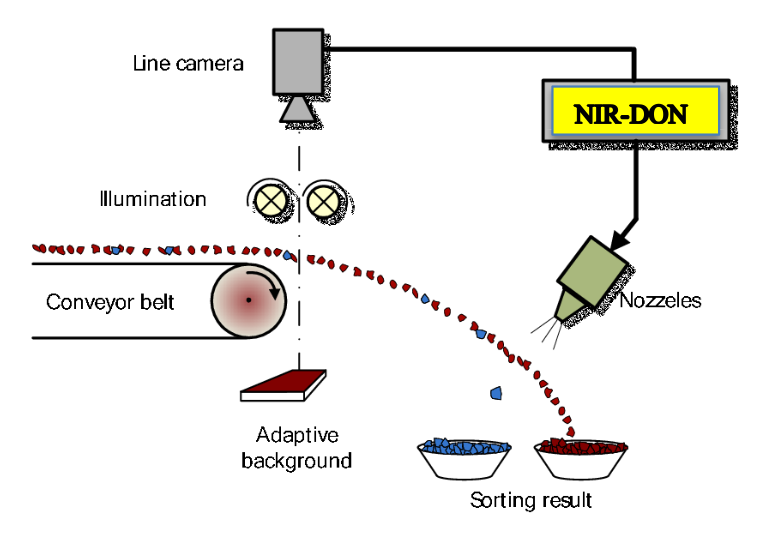
\includegraphics[width=0.7\linewidth]{media/images/esquema-del-sistema.png}
    \caption{Esquema del sistema de detección y filtrado de granos contaminados}\ \label{fig:detection-system}
\end{figure}


\subsection{NIR-HSI}


\gls{nir-hsi} es una tecnología rápida, no destructiva y precisa que nos permite hacer inspecciones de calidad, la cual ha demostrado su potencial en los últimos años\ \cite{Applicat5:online}. 
Es una técnica de imagen química basada en la espectroscopia de reflectancia (la luz reflejada por los materiales), la cual es capaz de caracterizar compuestos orgánicos y algunos minerales\ \cite{NIRHyper23:online}. Este método puede resultar mucho más directo, pues es rápido y no requiere análisis químico; barato, por los mismos motivos; y preciso, pues permite analizar los granos individualmente y no en lote; que el análisis químico.

Como hemos comentado en la introducción, nuestro objetivo es conseguir un modelo que, utilizando \gls{nir-hsi}, prediga lo mejor posible qué granos de una \gls{imagen hiperespectral} contienen granos contaminados con \acrshort{don}. Para ello, partimos con una base de datos de imágenes hiperespectrales con formato \acrshort{bil}, las cuales simulan las imágenes tomadas en la cadena de producción y de las cuáles podemos extraer la información de los píxeles que forman los granos.
Los archivos con formato \acrshort{bil} albergan los datos hiperespectrales de una imagen, como podemos ver en la \textit{figura \ref{fig:bil-example}}. Es decir, para las diferentes bandas especificadas, contiene la información de cada píxel que forma la imagen. Para ello, hace uso de otro archivo complementario con formato \textit{bil.hdr} que brinda información sobre este, como las diferentes bandas (frecuencias, en nuestro caso son 168) presentes en la imagen, entre otros. Una vez sabemos qué formato tienen los datos, podemos leer los archivos \acrshort{bil} que tenemos y formar un \acrshort{csv} con los datos centralizados para que nos sea más fácil trabajar con ellos. Para no tener un archivo demasiado grande, hemos desechado los píxeles que forman parte del `fondo' negro de la imagen, para determinar si un píxel es fondo, se hace la media de todos los valores de las reflectancias para ese píxel y si no pasa un umbral trivial, lo consideramos parte del fondo.

Una vez tenemos el \acrshort{dataset} con los datos de cada píxel, podemos generar un nuevo \acrshort{dataset} que agrupe los píxeles en grupos, o granos. De esta forma, podemos añadir un nuevo filtro que consista en que los granos deben de tener un tamaño mínimo (en píxeles), es decir, podemos desechar los granos que sean demasiado pequeños ya que probablemente sea ruido en la imagen. De esta forma, agruparíamos \textit{N} filas de datos de píxeles, en tan solo una fila conservando la media de cada columna.

\begin{figure}[!ht]
    \centering
    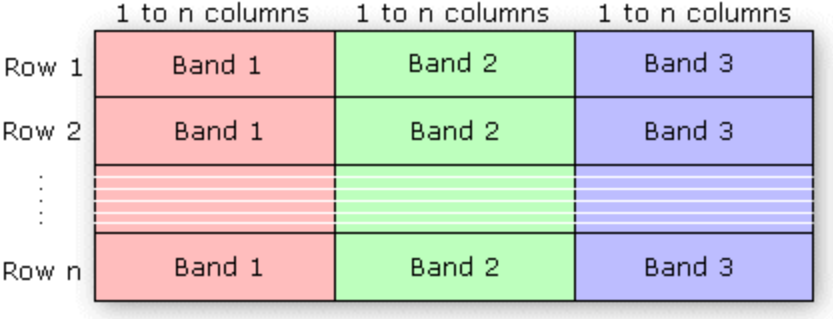
\includegraphics[width=0.7\linewidth]{media/images/bil.png}
    \caption{Formato de los datos en un archivo \acrshort{bil}. Fuente \cite{Archivos82:online}}\ \label{fig:bil-example}
\end{figure}

Por otro lado, tenemos una base de datos con el estado de contaminación de estos mismos granos. A partir de ahora utilizaremos los términos contaminación y etiqueta como sinónimos a la hora de referirnos a los granos.


\subsection{Contaminación del grano}\ \label{sec:separacion}

El valor de contaminación \acrshort{don} de una muestra se obtiene, como hemos comentado anteriormente, realizando un análisis químico por lotes. Este análisis nos devuelve el valor de la concentración de \acrshort{don} en el lote, de modo que si supera los \(1250\ \mu g/kg\), por ley, la muestra se considera contaminada. Sabiendo esto, previamente en laboratorio se ha realizado un análisis de los granos que forman las imágenes \acrshort{bil} que tenemos y, por lo tanto, además de los datos hiperespectrales, sabemos el nivel de contaminación que posee cada grano y lo podemos agregar como columna en el \acrshort{csv} que tenemos.


Al ser el valor de contaminación el que queremos predecir, a partir de ahora utilizaremos los términos contaminación y etiqueta como sinónimos. Además agregaremos otra columna, también de contaminación, la cual será \textit{booleana}, en lugar de un valor contínuo, y nos indicará si el valor concentración de ese grano supera el umbral legal comentado anteriormente. De esta forma, podemos plantear el problema tanto por regresión como por clasificación, 


\subsection{Análisis del mercado potencial}






\section{Marco teórico, conceptos clave del ML}

\begin{quote}
    `\gls{ml}: the use and development of computer systems that are able to learn and adapt without following explicit instructions, by using algorithms and statistical models to analyse and draw inferences from patterns in data'\ \cite{machinel18:online}
\end{quote}

Es decir, un sistema que es capaz de inferir patrones de unos datos y realizar predicciones sobre nuevos datos a raíz de los patrones encontrados. 


\subsection{Tipos de aprendizaje y modelos}

Hay cuatro tipos de aprendizaje en el ML:\@ supervisado, no supervisado, semi-supervisado y de refuerzo\ \cite{homl56}.

Como parte de nuestros datos están etiquetados, podemos utilizar tanto el aprendizaje supervisado como el semi-supervisado. En un sistema supervisado se requiere que todos los datos estén etiquetados con la categoría deseada, en nuestro caso la contaminación. Sin embargo, para el semi-supervisado no es necesario que todos los datos estén etiquetados, pues utilizan tanto los datos etiquetados como los que no (datos parcialmente etiquetados) para tratar de generalizar mejor\ \cite{homl56}.

No utilizaremos el no supervisado, pues consiste en un conjunto de técnicas utilizadas para agrupar automáticamente datos no etiquetados a base de similitudes sin tener supervisión previa. El objetivo es que los datos dentro de un mismo grupo sean más similares entre sí que con los otros grupos\ \cite{Clustera13:online}. Sin embargo, como tenemos una cantidad más o menos considerable de información etiquetada, no nos hace falta.

Tampoco utilizaremos el aprendizaje por refuerzo, pues no se encuentra implementado dentro de la librería que utilizamos \textit{\href{https://scikit-learn.org/stable/}{sklearn}} y tampoco está dentro de los objetivos del proyecto.


\subsection{Fases del desarrollo de un proyecto de ML}

Nuestro proyecto ha tenido las fases que nombramos a continuación:

\begin{enumerate}
    \item Obtención de datos (\textit{apartado\ \ref{sec:obtencion}})
        \begin{enumerate}
            \item Recolección de información de los \acrshort{bil}.
        \end{enumerate}
    \item Preparación de datos (\textit{apartado\ \ref{sec:preprocesado}})
        \begin{enumerate}
            \item Selección de métodos de preprocesado
        \end{enumerate}
    \item Entrenamiento de los modelos (\textit{apartado\ \ref{sec:entrenamiento}})
        \begin{enumerate}
            \item Entrenamiento `básico' de modelos
            \item Selección y refinamiento
        \end{enumerate}
    \item Evaluación de resultados
        
    \item Monitoreo de los modelos
\end{enumerate}

Podemos generalizar los procesos de un proyecto de \gls{ml} meidnate el esquema de la \textit{Figura\ \ref{fig:ml-development-cycle}}. Cabe destacar que el proceso de entrenar un modelo de \gls{ml}, como bien muestra la imagen, es un proceso cíclico en búsqueda de mejores resultados a base de probar metodologías distintas, añadir pasos, el cambio de requisitos, etc.

\begin{figure}[!htb]
    \centering
    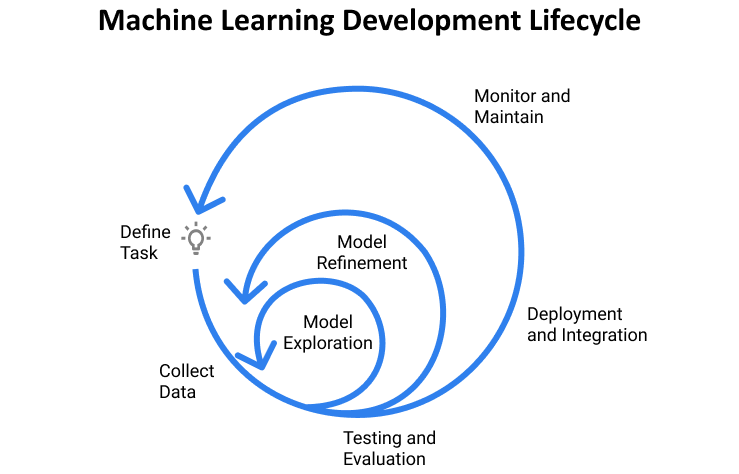
\includegraphics[width=\linewidth]{media/images/ml-development-cycle.png}
    \caption{Esquema del proceso del desarrollo de un proyecto de \gls{ml}, fuente\ \cite{Organizi22:online}}\ \label{fig:ml-development-cycle}
\end{figure}


\subsection{Métricas de evaluación de modelos}

Antes de continuar con el entrenamiento de modelos, su mejora y la selección de pasos del preprocesado; necesitamos algún tipo de métrica para evaluar y comparar los resultados. A continuación, explicaremos las que hemos utilizado para los diferentes tipos de modelos.

\subsubsection{Clasificación supervisada y semi-supervisada}\ \label{sec:classification-metrics}

Primeramente, explicaremos las partes de una matriz de confusión como la que podemos ver en la \textit{Figura\ \ref{fig:confusion-matrix-example}}. Podemos ver que tiene cuatro partes:

\begin{itemize}
    \item \textit{True Positive (tp)}, las muestras que el modelo clasifica como positivas que realmente son positivas.
    \item \textit{False Positive (fp)}, las muestras que el modelo clasifica como positivas que realmente son negativas.
    \item \textit{True Negative (tn)}, las muestras que el modelo clasifica como negativas que realmente son negativas.
    \item \textit{False Negative (fn)}, las muestras que el modelo clasifica como negativas que realmente son positivas.
\end{itemize}

Estos cuatro valores son la base del resto de métricas que comentaremos a continuación.

\begin{figure}[!ht]
    \centering
    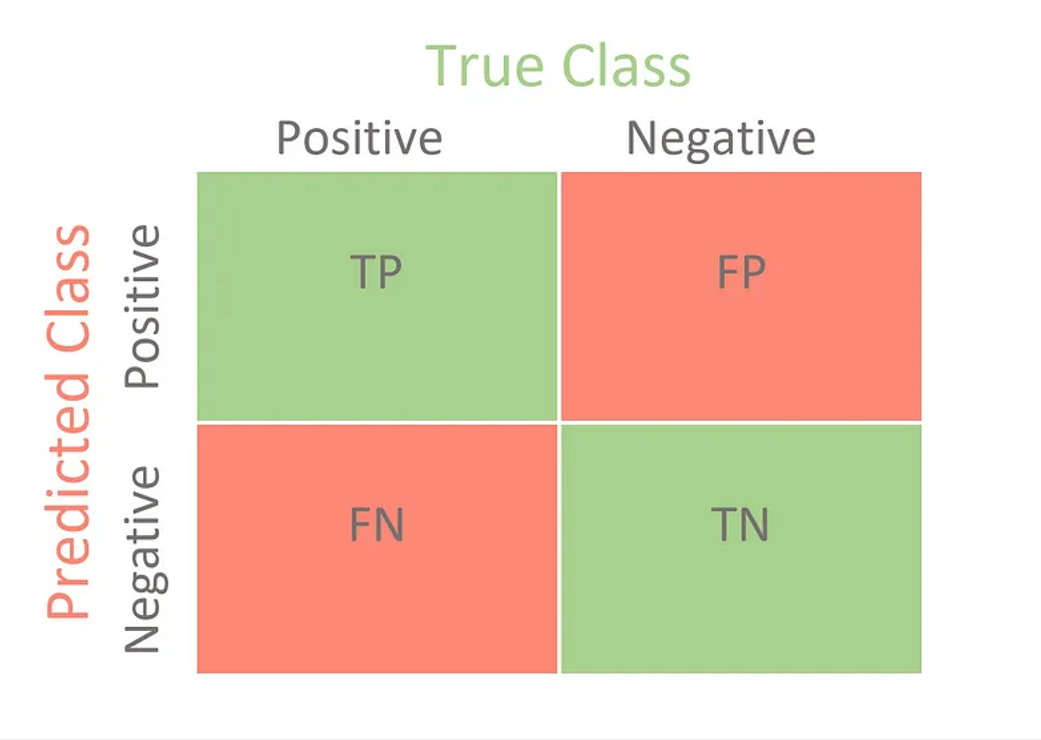
\includegraphics[width=0.7\linewidth]{media/images/confusion-matrix-example.png}
    \caption{Ejemplo de matriz de confusión, fuente\ \cite{Confusio71:online}}\ \label{fig:confusion-matrix-example}
\end{figure}

Antes de continuar con las métricas que compararemos, comentaremos también otras más básicas que son utilizadas para calcular las que utilizaremos\ \cite{Precisio23:online}.
\\ \textit{\textbf{Sensitivity}} permite saber la probabilidad de que una predicción positiva sea realmente positiva.
    \begin{equation}
        sensitivity=tp/(tp+fn)
    \end{equation}
\textit{\textbf{Specificity}} permite saber la probabilidad de que una predicción negativa sea realmente negativa.
\begin{equation}
        specificity=tn/(tn+fp)
    \end{equation}
\textit{\textbf{Recall}} indica la capacidad del modelo para encontrar todas las muestras positivas. 
    \begin{equation}
        recall=tp/(tp+fn)
    \end{equation}
\textit{\textbf{Precision}} indica la precisión de las predicciones positivas, es decir, la habilidad del clasificador para no predecir como positiva una muestra que es negativa.
    \begin{equation}
        precision=tp/(tp+fp)
    \end{equation}

Con estas métricas básicas podemos definir las que realmente compararemos, ya que tienen en cuenta el balanceo del \gls{dataset}:

\textit{\textbf{fbeta score}} es la media harmónica ponderada entre \textit{\textbf{Precision}} y \textit{Recall}. 
El parámetro \textit{beta} representa la importancia de \textit{Recall} por encima de \textit{Precision}. 
Es decir, \(beta>1\) le da más importancia a \textit{Recall} y, contrariamente, \(beta<1\) le da más peso a \textit{Precision}.\ \cite{FscoreWi30:online}
    \begin{equation}
        f_\beta = (1 + \beta^2)*\frac{precision*recall}{(\beta^2*precision)+recall}
    \end{equation}

Para comparar los modelos utilizaremos el parámetro \textit{beta} con valor de \textit{2}, pues consideramos más importante el \textit{Recall}, ya que creemos que los falsos negativos son peores que los falsos positivos. Es decir, consideramos peor que el modelo no detecte una muestra contaminada que detecte una muestra como contaminada cuando no lo es.

\textit{\textbf{Balanced accuracy}} es la media aritmética de \textit{Sensitivity} y \textit{Specificity}. Se utiliza principalmente cuando tratamos con datos desbalanceados.\ \cite{Balanced44:online} Su valor representa la exactitud media del modelo en las diferentes clases representadas por los datos, en nuestro caso, la clase de ``CONTAMINADO'' o ``NO CONTAMINADO''. Este valor, representa la exactitud con la que el modelo es capaz de clasificar las muestras de las diferentes clases, teniendo en cuenta la distribución de la clase mayoritaria. Es decir, si el valor de \textit{balanced accuracy} se acerca al 1, el modelo es capaz de clasificar correctamente las muestras de las diferentes clases, mientras que si se acerca a 0, el modelo no es capaz de clasificar correctamente las muestras o se aprovecha del desbalance de los datos, prediciendo mucho más la clase mayoritaria.
\begin{equation}
    balanced\_accuracy =\frac{sensitivity + specificity}{2}
\end{equation}

\section{Diseño del proyecto, primera iteración}

\subsection{Análisis del problema y de los datos}\label{sec:obtencion}

Considerando que los datos contenidos en los archivos \gls{bil} que hemos recibido desde el laboratorio contienen 168 columnas con información de las diferentes longitudes de onda\ \cite{WhatIsHy18:online} y además el nivel de contaminación \gls{don} de cada grano, podemos generar un \gls{dataset} con los datos de cada grano, haciendo la media de cada longitud de onda por cada píxel del mismo grano. Una vez hemos extraído la información de todos los archivos \gls{bil} y la hemos guardado en un archivo \acrshort{csv}, podemos entrenar los modelos.

Cabe recalcar que para los modelos de regresión hemos guardado el valor de contaminación \gls{don} explícitamente, para los de clasificación si el valor \gls{don} supera los límites de contaminación y hemos preparado un \gls{dataset} aparte con algunos archivos \gls{bil} que contienen granos que no han sido analizados químicamente para el entrenamiento semi-supervisado.

En esta primera iteración nos hemos centrado en intentar encontrar un buen modelo de clasificación y mejorar sus resultados lo máximo posible.

\subsection{Preprocesado de datos}\label{sec:preprocesado}

Ahora que tenemos los datos en un solo archivo \acrshort{csv}, el siguiente paso es preprocesarlos. Para ello, hemos realizado los siguientes pasos: 

\begin{enumerate}
    \item Eliminación de columnas
    \item Codificación
    \item Valores atípicos (\textit{outliers})
    \item Balanceo de datos
    \item Separación en datos de entreno y de prueba (\textit{train-test-split})
    \item Preprocesado común, (\textit{pipeline})
    \begin{enumerate}
        \item Separación de datos aplicando la primera derivada 
        \item Aumento de dimensionalidad (\textit{Polynomial Features})
        \item Estandarización  (\textit{Standard Scaler})
        \item Reducción de dimensionalidad (\textit{Principal Component Analysis})
    \end{enumerate}
    
\end{enumerate}


\subsubsection{Eliminación de columnas, codificación y valores atípicos}

Existen datos que nos interesan como medida de seguridad, pero no nos interesa que un modelo entrene con ellos, ya que podría inferir patrones irreales o incluso memorizárselos. En nuestro caso, un ejemplo sería una columna que indicase el número identificador del grano o el archivo del cual se han extraído los datos.

La codificación consiste en transformar columnas con datos categóricos en columnas de datos numéricos, pues los modelos de \acrshort{ml} funcionan mejor con valores numéricos. En nuestro caso, la única columna con valores no numéricos era la columna de la contaminación, que podía tomar los valores \textit{\{B, C\}}, así que lo codificamos manualmente como se muestra a continuación:

{\centering
    \textit{B \longrightarrow{} 0}, \textit{C \longrightarrow{} 1}\par
}

Los valores atípicos u \textit{outliers} son aquellos valores inusuales en los datos que pueden distorsionar nuestros análisis estadísticos. Sin embargo, se debe tener en cuenta que puede haber mucha variación en la naturaleza de nuestro problema. Por ello, se deben diferenciar los \textit{outliers} que se pueden incluir en los datos y los que no. En nuestro caso, los hemos incluido todos, pues al tener cada grano 168 columnas de datos, la mayoría tenía alguna columna que no entraba dentro de lo ``normal'', como por ejemplo en la \textit{figura\ \ref{fig:outliers}}. Por lo que después de probar a quitar todos los granos que alguna de sus columnas fuera un \textit{outlier} (con el \textit{código\ \ref{code:zscore}}), nos quedamos sin datos.

\begin{figure}[!h]
    \centering
    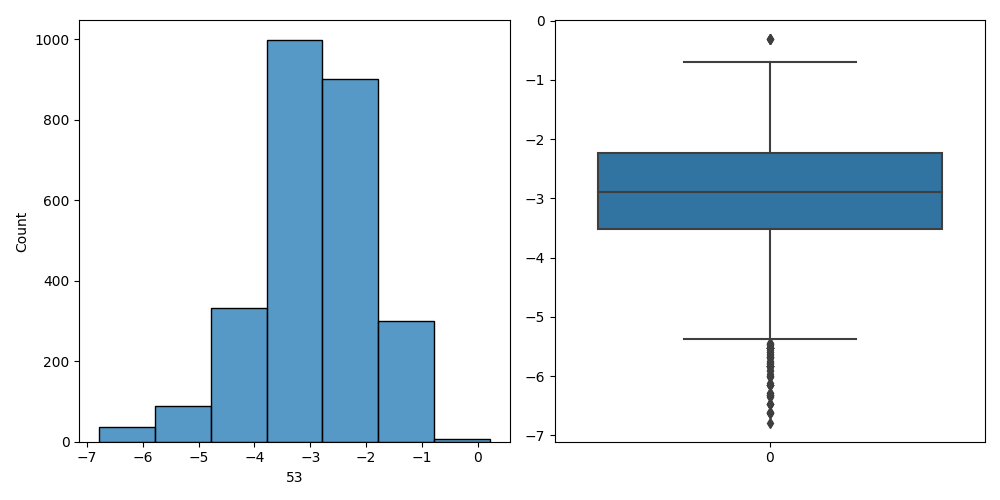
\includegraphics[width=0.7\linewidth]{media/images/col-53-outliers.png}
    \caption{Representación de los \textit{outliers} de la columna 53 en un gráfico de velas, fuente propia, \textit{código\ \ref{code:plot-outliers}}}\ \label{fig:outliers}
\end{figure}


\subsubsection{Balanceo de datos}

Podemos ver en la \textit{figura\ \ref{fig:unbalance}} que los datos no están balanceados, es decir, que la columna que nos interesa `Contaminación' no tiene un número de datos similares en cada clase. En nuestro caso, como en general es más complicado encontrarse un grano contaminado, tenemos más granos sanos.

Al tener las clases desbalanceadas tenemos varias opciones:
\begin{enumerate}
    \item Usar métodos de evaluación que tengan en cuenta el desbalance de las clases.
    \item Balancear el \gls{dataset} utilizando tanto \textit{undersampling} como \textit{oversampling} (explicados en el \textit{apartado\ \ref{sec:i2-balance}}).
\end{enumerate}

Para esta primera iteración, nos es más sencillo utilizar métricas que tengan en cuenta el número de instancias de cada clase a la hora de evaluar los resultados, es decir, que tengan en cuenta el desbalance del \gls{dataset}.

\begin{figure}[!h]
    \centering
    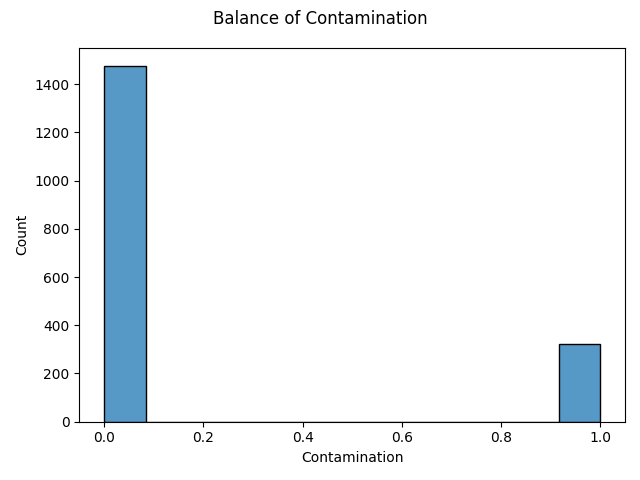
\includegraphics[width=0.7\linewidth]{media/images/unabalance.png}
    \caption{Balanceo de la clase objetivo del \gls{dataset}, fuente propia}\ \label{fig:unbalance}
\end{figure}


\subsubsection{Separación de datos de entreno y de prueba}

En todo el proyecto hemos estado utilizando la librería \href{https://scikit-learn.org/stable/}{sklearn}, esta tiene un submódulo con una función \href{https://scikit-learn.org/stable/modules/generated/sklearn.model_selection.train_test_split.html}{sklearn.model\_selection.train\_test\_split} para separar el \gls{dataset} en entreno y prueba. De todas las opciones, cabe recalcar una que hemos habilitado, pues como en el \gls{dataset} original las etiquetas no están balanceadas y hay muchos más granos sanos que contaminados, es importante que los granos contaminados estén igualmente representados tanto en el conjunto de prueba como en el de entreno. Esto se consigue con la opción \textit{stratify}.


\subsubsection{Preprocesado común}

Después de balancear los datos, debemos transformarlos para que tengan algunas propiedades que suelen ser preferibles a la hora de entrenar ciertos modelos. Es decir, hay modelos que les vendrá mejor tener los datos estandarizados, por ejemplo, y otros que no hará falta o será contraproducente, al final será la prueba y error lo que nos diga qué pasos son preferibles.

Antes de probar diferentes formas de preprocesar los datos, hemos preparado un entorno para entrenar una batería de modelos distintos para ver su efectividad.

Un primer paso, recomendado desde el laboratorio, ya que era lo que utilizaban ellos en su modelo estadístico, es aplicar la primera derivada. El aplicar la derivada permite mínimamente separar los granos contaminados de los que no. Para probarlo, podemos comparar los resultados de entrenar con o sin derivar en la \textit{tabla\ \ref{tab:nopreprocessing-derivative-results}} y, efectivamente, obtenemos resultados algo mejores.

\begin{table}[!h]
    \centering
    \resizebox{\textwidth}{!}{\begin{tabular}{|c|ccccccc|ccccccc|}
        \hline
        & \multicolumn{7}{|c|}{Derivative} & \multicolumn{7}{c|}{No preprocessing} \\ \hline
        Model Name & Train score & Test score & f1score & f0.5score & f2score & ROC/AUC score & Balanced accuracy & Train score & Test score & f1score & f0.5score & f2score & ROC/AUC score & Balanced accuracy \\ \hline
        XGBoost & 82 & 82 & 0 & 0 & 0 & 50 & 50 & 82 & 82 & 0 & 0 & 0 & 50 & 50 \\
        Stochastic Gradient Descent & 18 & 18 & 30.508 & 21.531 & 52.326 & 50 & 50 & 18 & 18 & 30.508 & 21.531 & 52.326 & 50 & 50 \\
        Random Forest & 99.926 & 87.778 & 49.541 & 69.948 & 38.352 & 66.531 & 66.531 & 99.556 & 84.889 & 52.778 & 57.057 & 49.096 & 70.069 & 70.069 \\
        Quadratic Discriminant Analysis & 100 & 82 & 0 & 0 & 0 & 50 & 50 & 100 & 82 & 0 & 0 & 0 & 50 & 50 \\
        Multi-Layer Perceptron & 83.259 & 80.667 & 8.421 & 14.599 & 5.917 & 51.114 & 51.114 & 82 & 82 & 0 & 0 & 0 & 50 & 50 \\
        Linear Discriminant Analysis & 85.333 & 78.222 & 20.968 & 25.692 & 17.711 & 53.96 & 53.96 & 84.889 & 78 & 22.047 & 26.415 & 18.919 & 54.306 & 54.306 \\
        LightGBM & 81.852 & 72 & 47.934 & 40 & 59.794 & 71.846 & 71.846 & 75.778 & 64 & 37.692 & 30.74 & 48.708 & 62.632 & 62.632 \\
        K-Neighbors & 100 & 86.889 & 56.296 & 63.973 & 50.265 & 71.289 & 71.289 & 100 & 91.778 & 74.83 & 79.71 & 70.513 & 82.46 & 82.46 \\
        Hist Gradient Boosting & 78.444 & 70.444 & 44.813 & 37.448 & 55.785 & 68.97 & 68.97 & 72.815 & 63.556 & 33.871 & 28.037 & 42.77 & 58.988 & 58.988 \\
        Extra Trees & 99.63 & 90.444 & 69.504 & 76.324 & 63.802 & 78.756 & 78.756 & 94.667 & 81.111 & 56.853 & 51.376 & 63.636 & 76.438 & 76.438 \\
        Decision Tree & 56.963 & 58.889 & 41.27 & 31.957 & 58.244 & 67.224 & 67.224 & 82 & 82 & 0 & 0 & 0 & 50 & 50 \\ \hline
        & & & & & & 61.79 & 61.79 & & & & & & 59.53572727 & 59.53572727 \\ \hline
        \end{tabular}}
    \caption{Comparación de los resultados de entrenar utilizando la derivada y sin preprocesar. Fuente propia.}\ \label{tab:nopreprocessing-derivative-results}
\end{table}


El siguiente paso que podemos probar es aplicar la transformada, como los resultados habiendo derivado los datos son mejores, transformaremos los datos después de derivarlos. Podríamos probar todas las permutaciones de los diferentes pasos de preprocesado, sin embargo, en esta primera iteración tan solo nos interesa encontrar un resultado decente. Podríamos hacerlo en una segunda o tercera iteración si lo vemos necesario. La transformada consiste en transformar cada columna para que tengan una forma gaussiana\ \cite{sklearnp39:online}. Como estamos utilizando \textit{sklearn}, tenemos una clase que nos aplica la transformada \href{https://scikit-learn.org/stable/modules/generated/sklearn.preprocessing.PowerTransformer.html}{sklearn.preprocessing.PowerTransformer}, por defecto esta clase además te aplica una estandardización de los datos, pero la hemos deshabilitado para aplicarla en otro paso. Podemos ver los resultados de entrenar utilizando la derivada y transformada en la \textit{tabla\ \ref{tab:derivative-transformed-results}}, podemos ver que los resultados son peores, así que continuaremos las pruebas con la derivada.

\begin{table}[!h]
    \centering
    \resizebox{\textwidth}{!}{\begin{tabular}{|c|ccccccc|ccccccc|}
        \hline
            & \multicolumn{7}{|c|}{Transformer and derivative} & \multicolumn{7}{c|}{Derivative} \\ \hline
            Model Name & Train score & Test score & f1score & f0.5score & f2score & ROC/AUC score & Balanced accuracy & Train score & Test score & f1score & f0.5score & f2score & ROC/AUC score & Balanced accuracy \\ \hline
            XGBoost & 82 & 82 & 0 & 0 & 0 & 50 & 50 & 82 & 82 & 0 & 0 & 0 & 50 & 50 \\
            Stochastic Gradient Descent & 18 & 18 & 30.508 & 21.531 & 52.326 & 50 & 50 & 18 & 18 & 30.508 & 21.531 & 52.326 & 50 & 50 \\
            Random Forest & 99.926 & 87.778 & 49.541 & 69.948 & 38.352 & 66.531 & 66.531 & 99.926 & 87.778 & 49.541 & 69.948 & 38.352 & 66.531 & 66.531 \\
            Quadratic Discriminant Analysis & 100 & 83.333 & 19.355 & 34.884 & 13.393 & 55.149 & 55.149 & 100 & 82 & 0 & 0 & 0 & 50 & 50 \\
            Multi-Layer Perceptron & 82 & 82 & 0 & 0 & 0 & 50 & 50 & 83.259 & 80.667 & 8.421 & 14.599 & 5.917 & 51.114 & 51.114 \\
            Linear Discriminant Analysis & 85.185 & 76.667 & 18.605 & 21.978 & 16.129 & 52.529 & 52.529 & 85.333 & 78.222 & 20.968 & 25.692 & 17.711 & 53.96 & 53.96 \\
            LightGBM & 81.852 & 72 & 47.934 & 40 & 59.794 & 71.846 & 71.846 & 81.852 & 72 & 47.934 & 40 & 59.794 & 71.846 & 71.846 \\
            K-Neighbors & 100 & 80.222 & 25.21 & 32.189 & 20.718 & 56.143 & 56.143 & 100 & 86.889 & 56.296 & 63.973 & 50.265 & 71.289 & 71.289 \\
            Hist Gradient Boosting & 78.444 & 70.444 & 44.813 & 37.448 & 55.785 & 68.97 & 68.97 & 78.444 & 70.444 & 44.813 & 37.448 & 55.785 & 68.97 & 68.97 \\
            Extra Trees & 99.63 & 90 & 68.966 & 74.184 & 64.433 & 78.967 & 78.967 & 99.63 & 90.444 & 69.504 & 76.324 & 63.802 & 78.756 & 78.756 \\
            Decision Tree & 56.963 & 58.889 & 41.27 & 31.957 & 58.244 & 67.224 & 67.224 & 56.963 & 58.889 & 41.27 & 31.957 & 58.244 & 67.224 & 67.224 \\ \hline
            & & & & & & 60.669 & 60.669 & & & & & & 61.79 & 61.79 \\ \hline
        \end{tabular}}
    \caption{Comparación de los resultados de entrenar transformando y derivando los datos; frente a solo derivando. Fuente propia.}\ \label{tab:derivative-transformed-results}
\end{table}

A continuación, probaremos la estandarización de los datos como hemos comentado anteriormente. Utilizaremos la clase \href{https://scikit-learn.org/stable/modules/generated/sklearn.preprocessing.StandardScaler.html}{sklearn.preprocessing.StandardScaler}.
La estandardización consiste en el centrado y escalado de los datos. Para ello, columna por columna, restamos la media de los valores (centramos en torno al 0) y 
los dividimos por la varianza (para que la desviación tienda a 1). Tener los datos estandarizados es suele ser un requisito para obtener buenos resultados al entrenar algunos modelos.\ \cite{sklearnp24:online}
Como consecuencia, en la \textit{tabla\ \ref{tab:derivative-standarization-results}} podemos ver que obtenemos mejores resultados.


\begin{table}[!h]
    \resizebox{\textwidth}{!}{\begin{tabular}{|c|ccccccc|ccccccc|}
        \hline
        & \multicolumn{7}{c|}{Derivative + Scaler} & \multicolumn{7}{c|}{Derivative} \\ \hline
        Model Name & Train score & Test score & f1score & f0.5score & f2score & ROC/AUC score & Balanced accuracy & Train score & Test score & f1score & f0.5score & f2score & ROC/AUC score & Balanced accuracy \\ \hline
        XGBoost & 82 & 82 & 0 & 0 & 0 & 50 & 50 & 82 & 82 & 0 & 0 & 0 & 50 & 50 \\
        Stochastic Gradient Descent & 64.815 & 56.444 & 24.615 & 20.075 & 31.809 & 49.834 & 49.834 & 18 & 18 & 30.508 & 21.531 & 52.326 & 50 & 50 \\
        Random Forest & 99.926 & 87.778 & 49.541 & 69.948 & 38.352 & 66.531 & 66.531 & 99.926 & 87.778 & 49.541 & 69.948 & 38.352 & 66.531 & 66.531 \\
        Quadratic Discriminant Analysis & 96.148 & 83.111 & 54.217 & 53.444 & 55.012 & 72.358 & 72.358 & 100 & 82 & 0 & 0 & 0 & 50 & 50 \\
        Multi-Layer Perceptron & 90.815 & 84 & 32.075 & 46.961 & 24.355 & 59.41 & 59.41 & 83.259 & 80.667 & 8.421 & 14.599 & 5.917 & 51.114 & 51.114 \\
        Linear Discriminant Analysis & 85.333 & 78.222 & 20.968 & 25.692 & 17.711 & 53.96 & 53.96 & 85.333 & 78.222 & 20.968 & 25.692 & 17.711 & 53.96 & 53.96 \\
        LightGBM & 82.222 & 72.222 & 48.133 & 40.222 & 59.917 & 71.981 & 71.981 & 81.852 & 72 & 47.934 & 40 & 59.794 & 71.846 & 71.846 \\
        K-Neighbors & 100 & 86.889 & 55.639 & 64.014 & 49.202 & 70.807 & 70.807 & 100 & 86.889 & 56.296 & 63.973 & 50.265 & 71.289 & 71.289 \\
        Hist Gradient Boosting & 78.444 & 70.444 & 44.813 & 37.448 & 55.785 & 68.97 & 68.97 & 78.444 & 70.444 & 44.813 & 37.448 & 55.785 & 68.97 & 68.97 \\
        Extra Trees & 99.63 & 90.444 & 69.504 & 76.324 & 63.802 & 78.756 & 78.756 & 99.63 & 90.444 & 69.504 & 76.324 & 63.802 & 78.756 & 78.756 \\
        Decision Tree & 56.963 & 58.889 & 41.27 & 31.957 & 58.244 & 67.224 & 67.224 & 56.963 & 58.889 & 41.27 & 31.957 & 58.244 & 67.224 & 67.224 \\ \hline
        & & & & & & 64.53009091 & 64.53009091 & & & & & & 61.79 & 61.79 \\ \hline
        \end{tabular}}
    \caption{Comparación de los resultados de entrenar derivando y estandarizando los datos; frente a solo derivando. Fuente propia.}\ \label{tab:derivative-standarization-results}
\end{table}


Además, podemos probar dos últimos pasos que suelen ir juntos. El primero, \href{https://scikit-learn.org/stable/modules/generated/sklearn.preprocessing.PolynomialFeatures.html}{sklearn.preprocessing.PolynomialFeatures}, 
nos permite generar nuevas columnas de datos que consisten en combinar las demás columnas, multiplicándolas entre sí y elevando a un grado específico (segundo grado en nuestro caso). 
De esta forma, teníamos un \gls{dataset} de 168 columnas y obtenemos uno de 14365 columnas. Por ello, debemos aplicar el segundo y último paso para reducir la dimensionalidad
de los datos. Este paso es \href{https://scikit-learn.org/stable/modules/generated/sklearn.decomposition.PCA.html}{sklearn.decomposition.PCA} o \textit{Principal Component Analysis},
reduce la dimensionalidad proyectando los datos a una espacio de menor dimensionalidad. Explicar este proceso más detenidamente se va de nuestro objetivo, pero
aquí podemos leer algo más al respecto sobre \textit{PCA} en \ \cite{Principa62:online}.
Aun añadiendo complejidad de esta forma, podemos ver en la \textit{tabla\ \ref{tab:derivative-standarization-dimensionality-results}} que los resultados son mejores si
nos quedamos en el paso anterior.

\begin{table}[!h]
    \resizebox{\textwidth}{!}{\begin{tabular}{|c|ccccccc|ccccccc|}
        \hline
            & \multicolumn{7}{c|}{Derivative + Scaler + Polynomial Features + PCA} & \multicolumn{7}{c|}{Derivative + Scaler} \\ \hline
            Model Name & Train score & Test score & f1score & f0.5score & f2score & ROC/AUC score & Balanced accuracy & Train score & Test score & f1score & f0.5score & f2score & ROC/AUC score & Balanced accuracy \\ \hline
            XGBoost & 82 & 82 & 0 & 0 & 0 & 50 & 50 & 82 & 82 & 0 & 0 & 0 & 50 & 50 \\
            Stochastic Gradient Descent & 53.333 & 50.444 & 28.754 & 22.299 & 40.468 & 52.439 & 52.439 & 64.815 & 56.444 & 24.615 & 20.075 & 31.809 & 49.834 & 49.834 \\
            Random Forest & 99.926 & 85.778 & 38.462 & 57.803 & 28.818 & 61.939 & 61.939 & 99.926 & 87.778 & 49.541 & 69.948 & 38.352 & 66.531 & 66.531 \\
            Quadratic Discriminant Analysis & 80.889 & 80 & 40 & 42.017 & 38.168 & 63.234 & 63.234 & 96.148 & 83.111 & 54.217 & 53.444 & 55.012 & 72.358 & 72.358 \\
            Multi-Layer Perceptron & 87.778 & 81.778 & 19.608 & 30.303 & 14.493 & 54.682 & 54.682 & 90.815 & 84 & 32.075 & 46.961 & 24.355 & 59.41 & 59.41 \\
            Linear Discriminant Analysis & 82.741 & 81.111 & 6.593 & 12.397 & 4.491 & 50.903 & 50.903 & 85.333 & 78.222 & 20.968 & 25.692 & 17.711 & 53.96 & 53.96 \\
            LightGBM & 77.037 & 68.444 & 38.261 & 32.496 & 46.512 & 62.933 & 62.933 & 82.222 & 72.222 & 48.133 & 40.222 & 59.917 & 71.981 & 71.981 \\
            K-Neighbors & 100 & 83.778 & 42.52 & 50.943 & 36.486 & 64.092 & 64.092 & 100 & 86.889 & 55.639 & 64.014 & 49.202 & 70.807 & 70.807 \\
            Hist Gradient Boosting & 75.63 & 66 & 37.037 & 30.864 & 46.296 & 61.924 & 61.924 & 78.444 & 70.444 & 44.813 & 37.448 & 55.785 & 68.97 & 68.97 \\
            Extra Trees & 96.222 & 82.222 & 51.22 & 50.847 & 51.597 & 70.37 & 70.37 & 99.63 & 90.444 & 69.504 & 76.324 & 63.802 & 78.756 & 78.756 \\
            Decision Tree & 71.852 & 68.889 & 27.835 & 25.328 & 30.892 & 55.014 & 55.014 & 56.963 & 58.889 & 41.27 & 31.957 & 58.244 & 67.224 & 67.224 \\ \hline
            & & & & & & 58.86636364 & 58.86636364 & & & & & & 64.53009091 & 64.53009091 \\ \hline
        \end{tabular}} 
    \caption{Comparación de los resultados de entrenar derivando, estandarizando y ajustando la dimensionalidad de los datos; frente a solo derivando y estandarizando. Fuente propia.}\ \label{tab:derivative-standarization-dimensionality-results}
\end{table}

Por último, es necesario comentar que como tenemos dos aplicaciones (una para entrenar modelos y otra para predecir sobre archivos \gls{bil}),
debemos guardarnos no solo el orden con el que hemos aplicado estos pasos de preprocesado, sino los valores que se han ido ajustando a los datos.
Esto se debe a que cuando uno de estos pasos se aplica sobre los datos de entreno se ajusta a ellos de una u otra forma y realiza un desplazamiento, los datos que debemos guardarnos
son los correspondientes a este desplazamiento. Cada paso almacena sus parámetros, por ejemplo el \textit{StandardScaler} se guarda la media y la varianza de cada columna,
por lo tanto podríamos guardar cada paso con sus parámetros como un archivo binario. Sin embargo, hay una clase que nos ayuda tanto a aplicar el preprocesado como a guardarlo como un solo
archivo `unificado'.\ \textit{Pipeline} nos da la posibilidad de añadir 
una lista de pasos a aplicar secuencialmente sobre un \gls{dataset}. De esta forma aplica los pasos sobre los datos, ajustando los parámetros de cada uno y luego nos permite
guardar el propio \textit{pipeline}, guardando en el tanto el orden de los pasos que lo componen, como los parámetros que representan sus desplazamientos.\ \cite{sklearnp32:online}


\subsection{Entrenamiento de modelos, selección e \textit{hypertuning}}\ \label{sec:entrenamiento}

Ahora que hemos encontrado una combinación de pasos de preprocesado decente, podemos pasar al siguiente paso de selección de los modelos. Aunque hay muchos tipos de modelos 
preparados en la librería, cada uno funciona de una forma distinta. Podríamos investigar cuál funciona mejor con nuestros datos, sin embargo, como el \gls{dataset} que 
tenemos no es muy grande, podemos entrenar todos sin perder mucho tiempo y mirar cuál tiene mejores resultados. Podemos ver en la \textit{tabla\ \ref{tab:best-preprocessing}}
el resultado del mejor preprocesado que hemos encontrado hasta ahora.

\begin{table}[!h]
    \resizebox{\textwidth}{!}{\begin{tabular}{|c|ccccccc|}
        \hline
        & \multicolumn{7}{c|}{Derivative + Scaler} \\ \hline
        Model Name & Train score & Test score & f1score & f0.5score & f2score & ROC/AUC score & Balanced accuracy \\ \hline
        XGBoost & 82 & 82 & 0 & 0 & 0 & 50 & 50 \\
        Stochastic Gradient Descent & 64.815 & 56.444 & 24.615 & 20.075 & 31.809 & 49.834 & 49.834 \\
        Random Forest & 99.926 & 87.778 & 49.541 & 69.948 & 38.352 & 66.531 & 66.531 \\
        Quadratic Discriminant Analysis & 96.148 & 83.111 & 54.217 & 53.444 & 55.012 & 72.358 & 72.358 \\
        Multi-Layer Perceptron & 90.815 & 84 & 32.075 & 46.961 & 24.355 & 59.41 & 59.41 \\
        Linear Discriminant Analysis & 85.333 & 78.222 & 20.968 & 25.692 & 17.711 & 53.96 & 53.96 \\
        LightGBM & 82.222 & 72.222 & 48.133 & 40.222 & 59.917 & 71.981 & 71.981 \\
        K-Neighbors & 100 & 86.889 & 55.639 & 64.014 & 49.202 & 70.807 & 70.807 \\
        Hist Gradient Boosting & 78.444 & 70.444 & 44.813 & 37.448 & 55.785 & 68.97 & 68.97 \\
        Extra Trees & 99.63 & 90.444 & 69.504 & 76.324 & 63.802 & 78.756 & 78.756 \\
        Decision Tree & 56.963 & 58.889 & 41.27 & 31.957 & 58.244 & 67.224 & 67.224 \\ \hline
        & & & & & & 64.53009091 & 64.53009091 \\ \hline
    \end{tabular}}
    \caption{Resultados de entrenar con el mejor preprocesado encontrado. Fuente: propia.}\ \label{tab:best-preprocessing}
\end{table}


Una vez hemos entrenado estos modelos vemos que hay algunos que hacen \textit{overfitting}. 
El \textit{overfitting} ocurre cuando un modelo se ajusta demasiado a los datos con los que ha entrenado y no generaliza bien, es decir que predice mejor los datos con los 
que ha entrenado que datos nuevos.
El modelo con el que lo podemos ver más claramente es el \textit{KNeighbors}, vemos en la \textit{figura\ \ref{fig:lc-knn}} que, para cualquier cantidad de datos con los 
que entrenemos el modelo, siempre predecirá bien con los que ha entrenado y no tanto con los demás. Nuestro objetivo es intentar que ambos valores
no sean tan dispares y que sean lo más altos posibles, para ello haremos \textit{hyperparameter tuning}.

\begin{figure}[!h]
    \centering
    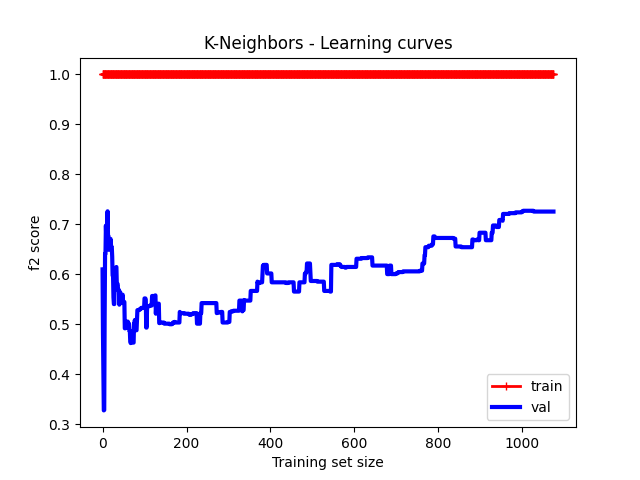
\includegraphics[width=0.7\linewidth]{media/images/learing-curves-knn.png}
    \caption{Gráfico de la curva de aprendizaje del modelo \textit{K-Neighbors} entrenándolo y probándolo sobre los datos de entreno únicamente. Fuente propia}\ \label{fig:lc-knn}
\end{figure}


\subsubsection{Selección de modelos e \textit{hyperparameter tuning}}\ \label{sec:i1-seleccion}

El \textit{hyperparameter tuning} tiene como objetivo encontrar un conjunto de parámetros que maximice el rendimiento del modelo. 
En nuestro caso, como los datos están desbalanceados, podemos utilizar como función de rendimiento el \textit{balanced accuracy}. 
Como cada modelo es distinto, debemos encontrar los parámetros adecuados para cada uno. 
Para ello, para ahorrarnos tiempo podemos utilizar solamente los mejores modelos, como hemos visto en los resultados de la \textit{tabla\ \ref{tab:best-preprocessing}}
hay modelos que tienen mejores resultados que otros.
Así que escogeremos los cuatro con mejor \textit{balanced accuracy}, es decir: \textit{Extra Trees, Quadratic Discriminant Analysis, LightGBM y K-Neighbors}.

Realizaremos el \textit{hyperparameter tuning} en dos pasos, primeramente utilizaremos \textit{Random Search} y después \textit{Grid Search}, ya implementados en \textit{sklearn}.
Ambos métodos utilizan \textit{cross-validation}, una técnica para evitar el \textit{overfitting} que consiste en la división de los datos de entreno en partes iguales.
Una vez dividido en \textit{N} partes, se entrena el modelo sobre todas las partes excepto una, la cual se utiliza para evaluar el modelo entrenado. Entonces, se repite el 
proceso cambiando de partición. De esta forma, haciendo la media obtenemos el resultado de entrenar el modelo repetidas ocasiones con los mismos parámetros, pero con datos 
distintos. Una vez hemos obtenido el mejor de los modelos que hemos entrenado, según la función de rendimiento, probamos el modelo resultante sobre los datos de prueba.
Podemos ver este proceso más gráficamente en la \textit{imagen\ \ref{fig:cross-validation}}.

\begin{figure}[!h]
    \centering
    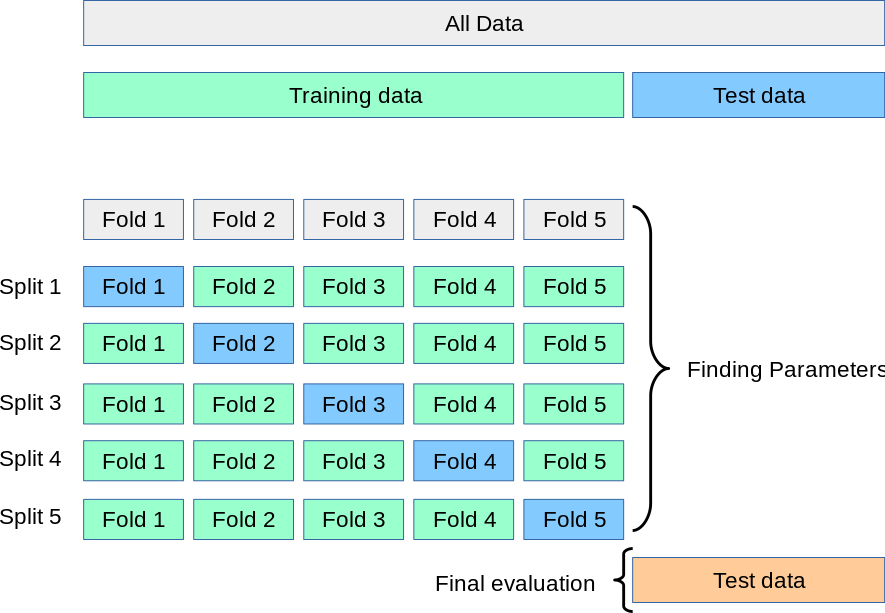
\includegraphics[width=0.7\linewidth]{media/images/cross-validation.png}
    \caption{\textit{Cross-validation} explicado gráficamente. Fuente:\ \cite{31Crossv20:online}}\ \label{fig:cross-validation}
\end{figure}


El \textit{random search} consiste en la búsqueda de estos parámetros habiendo definido un rango de posibilidades. Es decir, para cada parámetro que le queramos
pasar al modelo definiremos un rango de valores que puede tener, entonces el \textit{random search} entrena el modelo repetidas veces con una permutación aleatoria de sus 
parámetros y se guarda los resultados. Podemos ver un ejemplo en el \textit{código\ \ref{code:random-search-example}}.
Podemos ir probando diferentes parámetros y rangos hasta que estemos satisfechos con el resultado.


Una vez estemos contentos con los resultados, los refinaremos utilizando \textit{grid search}. A diferencia del \textit{random search}, el \textit{grid search} prueba todas
las posibles combinaciones que le pasemos como parámetro y, consecuentemente, es mucho más lento. Por ello, utilizaremos el \textit{grid search} con los mejores parámetros que
encontremos del paso anterior, los cuales son potencialmente los mejores. Una vez definido un rango de parámetros para los modelos seleccionados, obtenemos los resultados
de la \textit{tabla\ \ref{tab:hyperparameter-tuning-results}}. Podemos ver que hemos obtenido, en general, peores resultados (salvo con \textit{K-Neighbors}), por lo tanto
deberíamos ajustar el rango de parámetros que les pasamos a los modelos y volver a entrenarlos hasta que estemos satisfechos con el resultado. En nuestro caso no lo haremos
y pasaremos a la segunda iteración del proyecto para probar nuevas cosas en pasos anteriores.

\begin{table}
    \resizebox{\textwidth}{!}{\begin{tabular}{|c|ccccccc|}
            \hline
            Model name & Train score & Accuracy & f1 score & f0.5 score & f2 score & ROC/AUC score & Balanced accuracy \\ \hline
            RS - knn & 100 & 90.274 & 85.897 & 87.927 & 83.96 & 90.274 & 90.274 \\
            GS - knn & 100 & 90.274 & 85.897 & 87.927 & 83.96 & 90.274 & 90.274 \\
            RS - qda & 97.491 & 72.358 & 54.217 & 53.444 & 55.012 & 72.358 & 72.358 \\
            GS - qda & 97.491 & 72.358 & 54.217 & 53.444 & 55.012 & 72.358 & 72.358 \\
            RS - lgbm & 86.013 & 71.018 & 47.257 & 39.716 & 58.333 & 71.018 & 71.018 \\
            GS - et & 82.957 & 66.17 & 43.077 & 39.106 & 47.945 & 66.17 & 66.17 \\
            GS - lgbm & 84.628 & 70.626 & 46.215 & 38.108 & 58.704 & 70.626 & 70.626 \\
            RS - et & 69.492 & 65.854 & 40.909 & 33.21 & 53.254 & 65.854 & 65.854 \\\hline
            \end{tabular}
    }
    \caption{Resultados del primer entrenamiento con hyperparameter tuning. Fuente propia.}\ \label{tab:hyperparameter-tuning-results}
\end{table}


\section{Segunda iteración}

En esta segunda iteración pretendemos mejorar algunos de los aspectos que nos hemos encontrando en la primera, o aspectos que simplemente hemos dejado para después. Comenzaremos con una alternativa al balanceo de datos, y luego probaremos otros tipos tanto de aprendizaje como de modelos.

\subsection{Balanceo de datos}\ \label{sec:i2-balance}

La toma de nuevos datos es costosa y como tenemos relativamente pocos para la cantidad de columnas (las 168 longitudes de onda), el balanceo de datos es esencial. En la primera iteración, intentamos sortear este problema utilizando métricas que tienen en cuenta el balance de los datos. Sin embargo, podemos balancear los datos en dos pasos: \textit{undersampling} y \textit{oversampling}. 

Como su nombre indica, \textit{undersampling} es una técnica para reducir las muestras de la clase mayoritaria, en nuestro caso los granos sin contaminar. Existen varias técnicas para hacer \textit{undersampling}, las cuales comentaremos en la \textit{sección\ \ref{sec:undersampling}}. Por otro lado, el \textit{oversampling} consiste en la creación de datos sintéticos, similares a los reales, para suplir la diferencia de granos. Al igual que con el \textit{undersampling}, existen diversas técnicas que comentaremos más adelante en la \textit{sección\ \ref{sec:oversampling}}.


\subsubsection{\textit{Undersampling}}\ \label{sec:undersampling}

A la hora de balancear los datos, buscamos, de alguna forma, reducir la diferencia en el número de muestras en las diferentes clases. En el paso de \textit{undersampling}, buscamos reducir la cantidad de muestras de las clases mayoritarias, recordamos que nuestro caso lo podemos ver en la \textit{figura\ \ref{fig:unbalance}}. Para ello, debemos de alguna forma determinar qué muestras de las clases mayoritarias son más redundantes para evitar eliminar muestras `críticas'. Comentaremos a continuación diferentes algoritmos que nos ayudan con este paso.

Los algoritmos que hemos decidido utilizar son los de la librería \href{https://imbalanced-learn.org/stable/}{imblearn} que fue diseñada específicamente para los problemas de clasificación sobre \textit{datasets} desbalanceados.\ \cite{3Undersa98:online}

El primer algoritmo que probaremos será \textit{RandomUnderSampler}, el cual consiste en seleccionar un subconjunto aleatorio de datos. Para intentar no eliminar datos importantes como hemos comentado antes, hay otra versión que aplica una de las tres versiones de la heurística \textit{NearMiss}\ \cite{3Undersa98:online}, la cual se basa en el algoritmo \textit{nearest neighbors}:

\begin{enumerate}
    \item La versión \textbf{1} elimina aquellos datos cuya distancia media a sus \textit{N} vecinos más cercanos de la clase minoritaria sea menor.
    \item La versión \textbf{2} es parecida a la \textbf{1}, pero en esta la distancia media se computa sobre los \textit{N} vecinos más lejanos de la clase minoritaria.
    \item La versión \textbf{3} consta de dos pasos, primero de cada elemento de la clase minoritaria selecciona los \textit{M} vecinos más cercanos de la clase mayoritaria. Luego, por cada muestra seleccionada se calcula la distancia media respecto a los \textit{N} vecinos más cercanos de la clase minoritaria y se eliminan los que, de media, estén más alejados.
\end{enumerate}

El algoritmo \textit{Tomek Links} detecta los llamados \textit{Tomek Links}, estos son enlaces entre dos muestras de diferente clase, pongamos \(x\) e \(y\), definidos tal que para cualquier muestra \(z\): 
\[d(x,y) < d(x,z)\ and\ d(x,y) < d(y,z)\], donde \(d(a, b)\) es la distancia entre la muestra \(a\) y \(b\). En resumen, un \textit{Tomek Link} se da entre las muestras de distintas clases más cercanas entre sí. Este algoritmo suele ser bueno a la hora de eliminar ruido en los datos.

\textit{Edited Nearest Neighbours} en resumen elimina las muestras que no se parezcan demasiado a sus vecinos\ \cite{Wil72}. Para ello, comprueba para cada muestra que sus \textit{N} vecinos más cercanos sean de su misma clase, y si no podemos elegir si nos quedamos con la mayoría o si eliminamos todas las muestras.

Podemos ver los resultados de entrenar los modelos básicos que hemos probado anteriormente sobre los \textit{dataset} reducidos con los métodos comentados en la \textit{tabla\ \ref{tab:undersampling-methods}}. Podemos ver que, generalmente, el algoritmo \textit{Near Miss} es el que mejor funciona, aunque cabe destacar que, como podemos ver en la \textit{figura\ \ref{fig:undersampling-methods-balance}}, el algoritmo \textit{Near Miss} reduce mucho más la cantidad de datos.

\begin{table}[!ht]
    \resizebox{\textwidth}{!}{\begin{tabular}{|c|ccc|} \hline
        & Avg. f0.5 Score & Avg. f2 Score & Avg. Balanced Accuracy \\ \hline
        Random Under Sampler & 61.0523 & 59.2609 & 62.6545 \\
        Near Miss (v1) & 70.2289 & 66.7329 & 69.6297 \\
        Near Miss (v2) & 74.6031 & 68.1454 & 73.0865 \\
        Near Miss (v3) & 67.7945 & 71.1278 & 64.9608 \\
        Edited Nearest Neighbors (ALL) & 48.8632 & 47.0348 & 67.8832 \\
        Edited Nearest Neighbors (MODE) & 44.4157 & 41.1859 & 64.5333 \\
        Tomek Links & 41.5187 & 41.1415 & 64.6431 \\ \hline
        \end{tabular}}
    \caption{Resultado de entrenar los modelos básicos sobre el \textit{dataset} reducido con los diferentes métodos. Fuente: propia.}\ \label{tab:undersampling-methods}
\end{table}

\begin{figure}[!ht]
    \centering
    \begin{subfigure}[b]{0.5\textwidth}
        \centering
        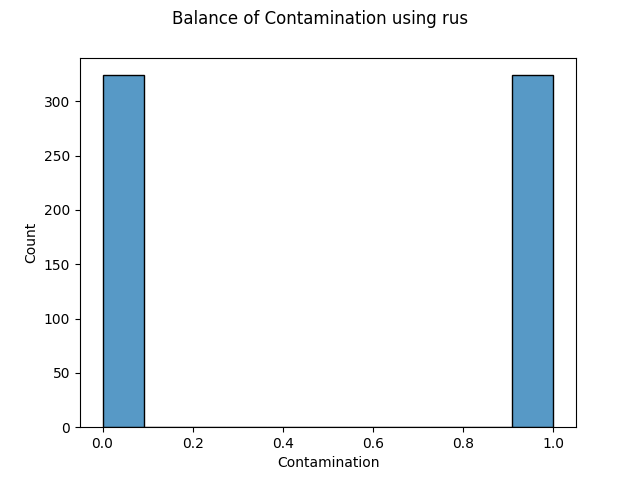
\includegraphics[width=\textwidth]{media/images/under-sampling/rus.png}
        \caption{Comparación del balance utilizando \textit{Random Under Sampler}}
    \end{subfigure}%
    \begin{subfigure}[b]{0.5\textwidth}
        \centering
        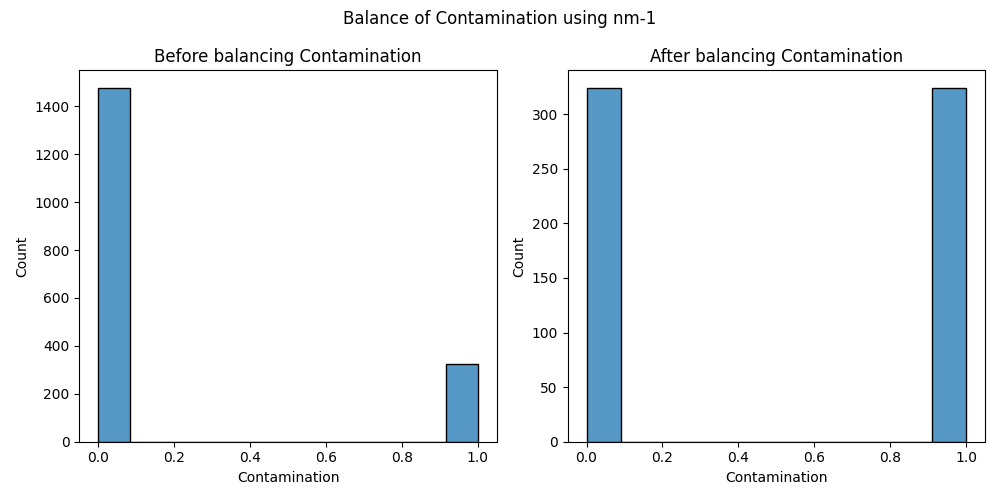
\includegraphics[width=\textwidth]{media/images/under-sampling/nm-1.png}
        \caption{Comparación del balance utilizando \textit{Near Miss 1}}
    \end{subfigure}
    \begin{subfigure}[b]{0.5\textwidth}
        \centering
        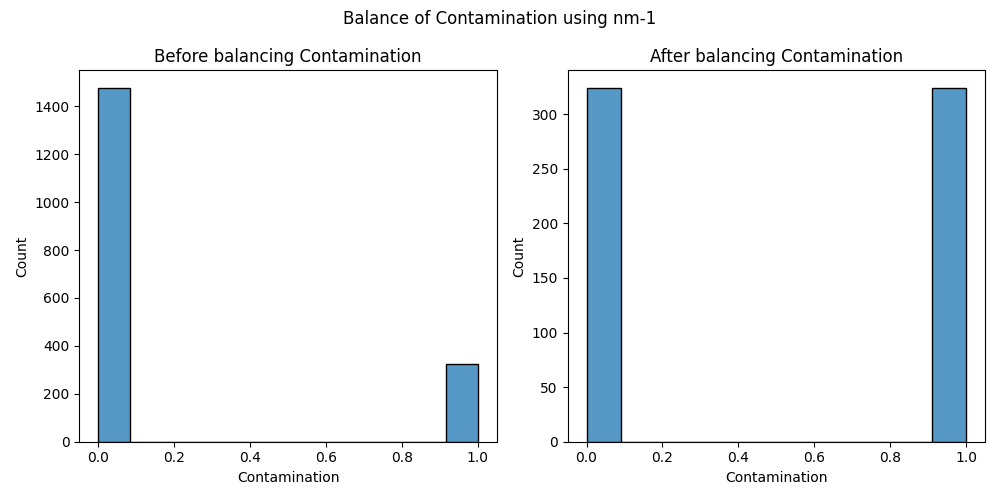
\includegraphics[width=\textwidth]{media/images/under-sampling/nm-1.png}
        \caption{Comparación del balance utilizando \textit{Near Miss 2}}
    \end{subfigure}%
    \begin{subfigure}[b]{0.5\textwidth}
        \centering
        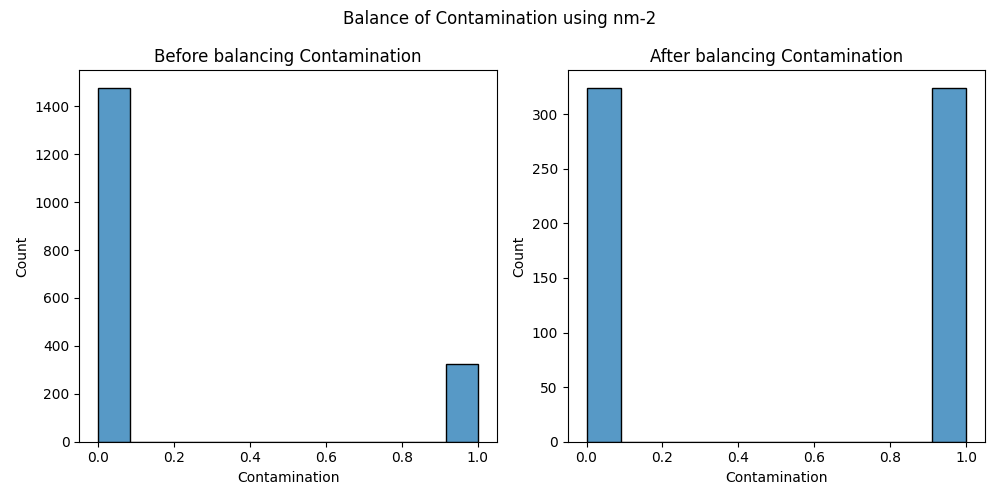
\includegraphics[width=\textwidth]{media/images/under-sampling/nm-2.png}
        \caption{Comparación del balance utilizando \textit{Near Miss 3}}
    \end{subfigure}
    \begin{subfigure}[b]{0.5\textwidth}
        \centering
        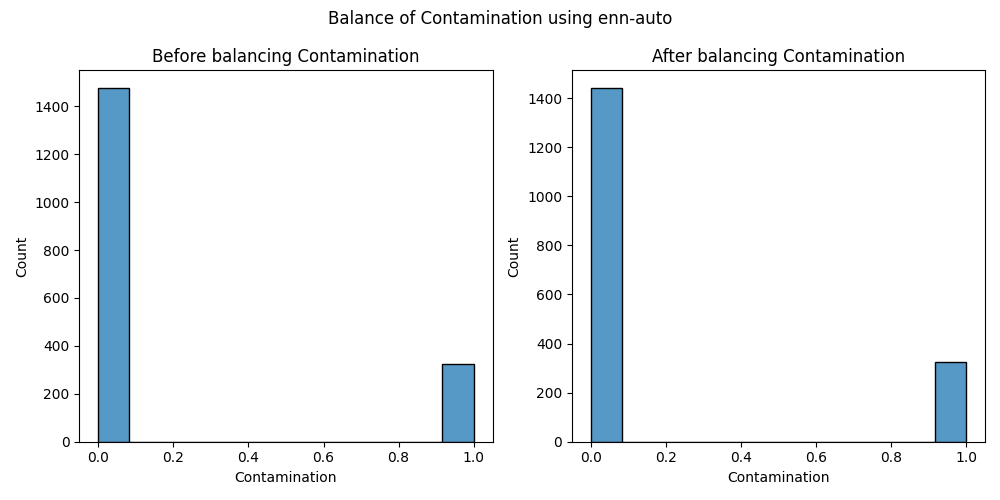
\includegraphics[width=\textwidth]{media/images/under-sampling/enn-auto.png}
        \caption{Comparación del balance utilizando \textit{Edited Nearest Neighbors (AUTO)}}
    \end{subfigure}%
    \begin{subfigure}[b]{0.5\textwidth}
        \centering
        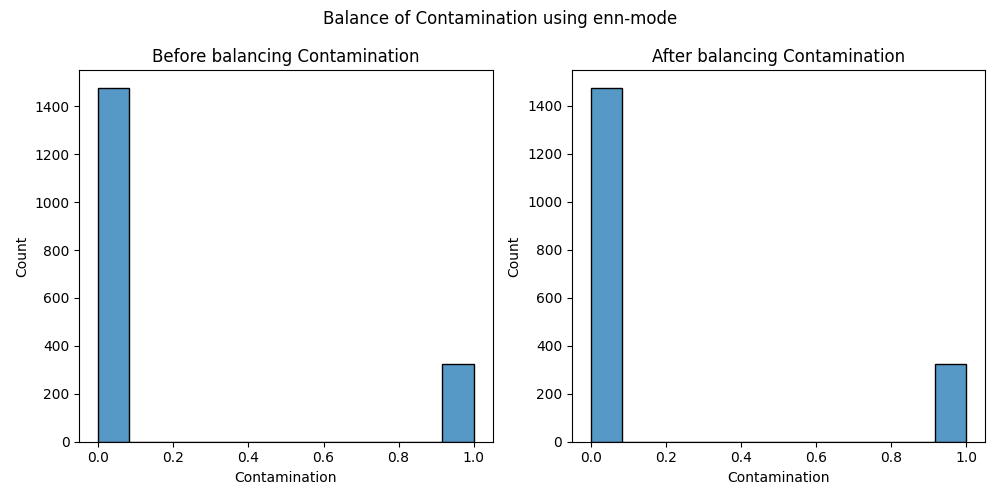
\includegraphics[width=\textwidth]{media/images/under-sampling/enn-mode.png}
        \caption{Comparación del balance utilizando \textit{Edited Nearest Neighbors (MODE)}}
    \end{subfigure}
    \begin{subfigure}[b]{0.5\textwidth}
        \centering
        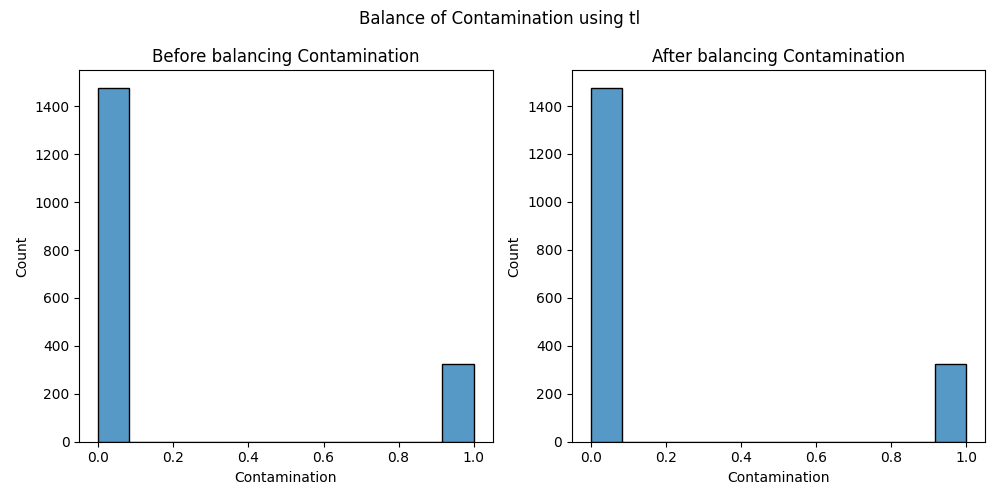
\includegraphics[width=\textwidth]{media/images/under-sampling/tl.png}
        \caption{Comparación del balance utilizando \textit{Tomek Links}}
    \end{subfigure}
    \caption{Comparaciones del balance de los \textit{dataset} utilizando los diferentes algoritmos de \textit{undersampling}.}\label{fig:undersampling-methods-balance}
\end{figure}
\clearpage

\subsubsection{\textit{Oversampling}}\ \label{sec:oversampling}

El segundo paso es el \textit{oversampling}, el cual consiste en la creación de los datos sintéticos para suplir la carencia de datos de una clase minoritaria. Hay algoritmos para realizar estas técnicas implementados en \textit{imblearn}, sin embargo preferimos utilizar \href{https://sdv.dev/}{sdv}, pues tiene mejor documentación y tiene un método `fácil' para evaluar los datos generados. \cite{Synthesi69:online} En general, los sintetizadores utilizan algoritmos complejos sobre los cuales podemos leer en \cite{Synthesi69:online}, pero para agilizar el proceso de análisis no entraremos demasiado en detalle.

Antes de comentar los sintetizadores que probaremos, comentaremos el método de evaluación de los datos generados con los que los evaluaremos. Utilizaremos una función de la propia librería \textit{sdv} que evalúa la similitud estadística de los datos generados con los datos reales.

Los tres sintetizadores que probaremos son:

\begin{enumerate}
    \item \textit{Gaussian Copula Synthesizer} \cite{Gaussian4:online}, el cual utiliza unos métodos clásicos estadísticos.
    \item \textit{CTGANSynthesizer} \cite{CTGANSyn50:online}, utiliza métodos de \textit{deep learning} basados en \textit{GAN} \cite{Generati72:online}.
    \item \textit{TVAESynthesizer} \cite{TVAESynt0:online}, basado en \textit{VAE} \cite{Variatio61:online}, utiliza técnicas de redes neuronales.
\end{enumerate}

Habiéndolos entrenado, evaluaremos su similitud con los datos reales y nos quedaremos con el más semejante.


\begin{figure}[!ht]
    \centering
    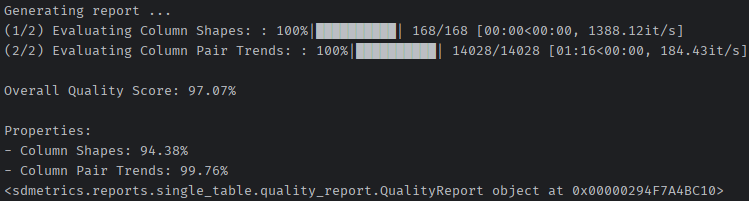
\includegraphics[width=0.8\linewidth]{media/images/quality_report.png}
    \caption{Reporte de calidad de los datos generados sintéticamente, fuente propia.}\ \label{fig:quality_report}
\end{figure}

Una vez aplicados los dos algoritmos obtenemos un \gls{dataset} balanceado como el de la \textit{figura\ \ref{fig:balance}}.

La toma de nuevos datos reales es costosa, y como teníamos relativamente pocos datos para entrenar el balanceo es esencial. Podemos hacer unos entrenamientos y comparar los resultados para ver si es necesario 
balancear, los resultados los podemos ver en la \textit{tabla\ \ref{tab:balanced_comparison}}. Fijándonos en las columnas a partir de \textit{f1score}, ya que estas son las métricas que ignoran el balanceo de 
los datos, podemos ver que, son mejores los modelos entrenados sobre el \gls{dataset} balanceado.

\begin{table}[!ht]
    \centering
    \resizebox{\textwidth}{!}{\begin{tabular}{|c|ccccc|ccccc|} \hline
    & \multicolumn{5}{|c|}{Balanced dataset} & \multicolumn{5}{c|}{Unbalanced dataset} \\ \hline
        Model Name & Train score & Test score & f1score & f0.5score & Balanced accuracy & Train score & Test score & f1score & f0.5score & Balanced accuracy \\ \hline
        XGBoost model & 92.051 & 87.669 & 87.055 & 89.736 & 87.669 & 82 & 82 & 0 & 0 & 50 \\
        Stochastic Gradient Descent & 79.584 & 78.862 & 76.506 & 81.988 & 78.862 & 64.815 & 56.444 & 24.615 & 20.075 & 49.834 \\
        Random Forest model & 94.399 & 87.398 & 86.58 & 90.09 & 87.398 & 99.926 & 87.778 & 49.541 & 69.948 & 66.531 \\
        Quadratic Discriminant Analysis & 87.94 & 87.669 & 86.191 & 92.871 & 87.669 & 96.148 & 83.111 & 54.217 & 53.444 & 72.358 \\
        Multi-Layer Perceptron & 89.205 & 85.908 & 85.014 & 88.376 & 85.908 & 90.815 & 84 & 32.075 & 46.961 & 59.41 \\
        Linear Discriminant Analysis & 82.746 & 80.759 & 78.743 & 84.026 & 80.759 & 85.333 & 78.222 & 20.968 & 25.692 & 53.96 \\
        LightGBM model & 92.141 & 87.127 & 86.409 & 89.402 & 87.127 & 82.222 & 72.222 & 48.133 & 40.222 & 71.981 \\
        K-Neighbors model & 100 & 83.333 & 81.048 & 88.314 & 83.333 & 100 & 86.889 & 55.639 & 64.014 & 70.807 \\
        Hist Gradient Boosting model & 82.294 & 81.436 & 79.764 & 84.322 & 81.436 & 78.444 & 70.444 & 44.813 & 37.448 & 68.97 \\
        Extra Trees model & 86.224 & 84.688 & 82.695 & 89.701 & 84.688 & 99.63 & 90.444 & 69.504 & 76.324 & 78.756 \\
        Decision Tree model & 80.352 & 79.268 & 76.279 & 83.503 & 79.268 & 56.963 & 58.889 & 41.27 & 31.957 & 67.224 \\ \hline
    \end{tabular}}
    \caption{Tabla comparativa de los resultados de entrenar los modelos con los datos balanceados y sin balancear, después de preprocesar los datos. Fuente propia.}\ \label{tab:balanced_comparison}
\end{table}


\begin{figure}[!ht]
    \centering
    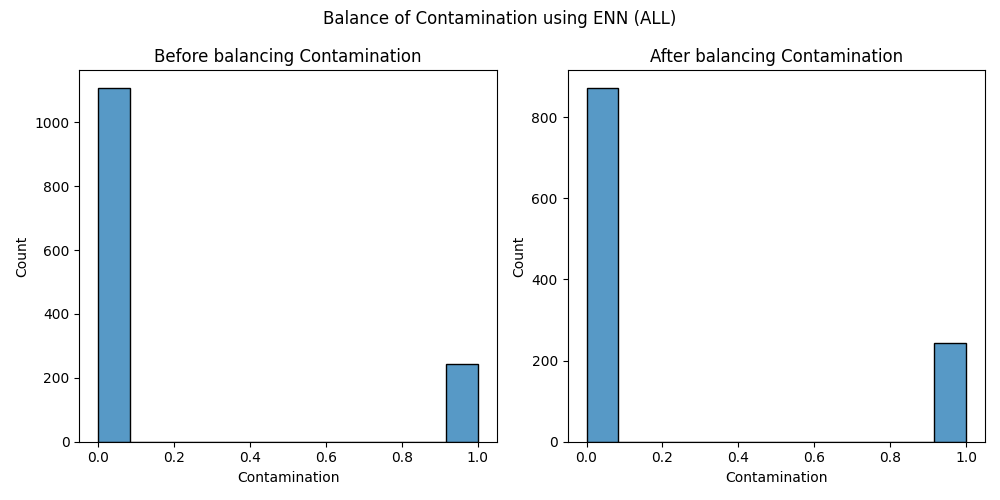
\includegraphics[width=0.6\linewidth]{media/images/balance.png}
    \caption{Comparación del balanceo de la clase objetivo del \gls{dataset} antes y después de balancear, fuente propia, código\ \ref{code:plots_balancing}}\ \label{fig:balance}
\end{figure}
\section{Resultados y conclusiones}

Durante el proyecto, hemos podido observar que los resultados han ido mejorando (generalmente) a medida que probábamos nuevas tecnologías. 
\include{sections/7-Discusión}
\section{Anexo}
\label{sec:anex}

\begin{figure}[!htb]
    \centering
    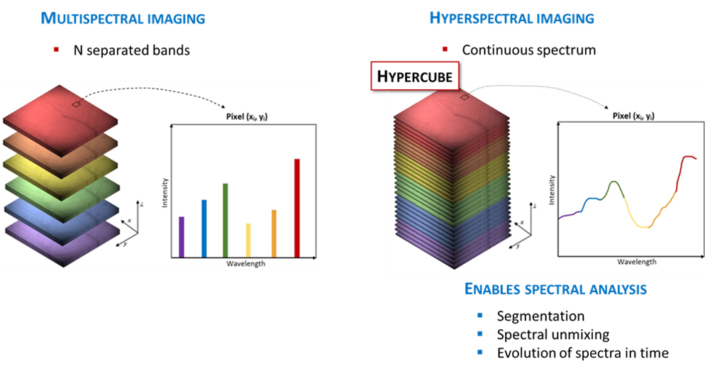
\includegraphics[width=0.7\linewidth]{media/images/hyperspectral_image.png}
    \caption{Esquemas para almacenar los valores de píxel reales de una imagen en un archivo \acrshort{bil}, referencia: \cite{Archivos82:online}}
    \label{fig:hyperspectral_image}
\end{figure}

\begin{code}[numbers=left]{title=Gráfico de velas de los outliers, label=code:plot-outliers}{Python}
def plots_outliers(outliers_df: pd.DataFrame, column=53):
    fig, axes = plt.subplots(ncols=2, figsize=(10, 5))
    sns.histplot(outliers_df[column], binwidth=1, ax=axes[0])
    sns.boxplot(outliers_df[column], ax=axes[1])
    fig.tight_layout()
    plt.show()
\end{code}

\begin{code}[numbers=left]{title=Detección de outliers utilizando \textit{zscore}, label=code:zscore}{Python}
...
    zscore = np.abs(stats.zscore(df))
    data_clean = df[(zscore < 3).all(axis=1)]
    df = data_clean
...
\end{code}

\begin{code}[numbers=left]{title=Gráfico de curvas de aprendizaje, label=code:plot-learning-curves}{Python}
def plots_balancing(df, df_balanced):
    fig, axis = plt.subplots(ncols=2, figsize=(10, 5))
    fig.suptitle(f'Balance of {src.utils.dev_config.OBJECTIVE_COLUMN}')
    axis[0].set_title(f'Before balancing {src.utils.dev_config.OBJECTIVE_COLUMN}')
    axis[1].set_title(f'After balancing {src.utils.dev_config.OBJECTIVE_COLUMN}')
    plot_balance(df, ax, 0)
    plot_balance(df_balanced, ax, 1)
    f.tight_layout()
    plt.show()
z

def plot_balance(df, axis, axis_number):
    return sns.histplot(df[src.utils.dev_config.OBJECTIVE_COLUMN], ax=axis[axis_number] if axis_number else axis)
\end{code}

\begin{code}[numbers=left]{title=Gráfico de comparación del balanceo, label=code:plots_balancing}{Python}
def plot_learning_curves(model, model_name, x, y):
    x_train, x_val, y_train, y_val = train_test_split(x, y, test_size=0.2)
    train_errors, val_errors = [], []
    
    for m in range(5, len(x_train)):
        model.fit(x_train[:m], y_train[:m])
        y_train_predict = model.predict(x_train[:m])
        y_val_predict = model.predict(x_val)
        train_errors.append(metrics.fbeta_score(y_train[:m], y_train_predict, beta=2))
        val_errors.append(metrics.fbeta_score(y_val, y_val_predict, beta=2))
        
    plt.title(f'{model_name} - Learning curves')
    plt.plot(np.sqrt(train_errors), "r-+", linewidth=2, label="train")
    plt.plot(np.sqrt(val_errors), "b-", linewidth=3, label="val")
    plt.xlabel("Training set size")
    plt.ylabel("f2 score")
    plt.legend(loc="best")
    plt.show()
\end{code}

% ---------------------------------------------------------- %
% 
\clearpage

% APPENDIX
% \subfile{sections/appendix}
% \clearpage

% SPECIAL TERMS
\printglossary[title=Definiciones adicionales, nonumberlist]\ \label{sec:additional-definitions}
\clearpage

% BIBLIOGRAPHY
\printbibliography[heading=bibintoc, title=Bibliografía y referencias]


\end{document}